\documentclass[10pt,twocolumn]{article}
	
\usepackage{myfontstyle}
\usepackage{mypackages}
\usepackage{mymacros}
\usepackage{mycommands}
\usepackage{graphicx}
\usepackage{hyperref}

\begin{document}
\thispagestyle{fancy1}

%%% Title and Abstract------------------------
\twocolumn[
\begin{center}
	\hrule
	\vspace{3pt}
	% Title:
	{\sffamily\bfseries\Large
		Report for Assignment 10: Function Approximation Showdown
	} \\
	{\color{gray}
		\vspace{3pt}
		\hrule
		\vspace{3pt}
	}
	{
		\hspace*{\fill}
		Julian Soh
		\hspace*{\fill}
%		Second Author
%		\hspace*{\fill}
%		Third Author
%		\hspace*{\fill}
%		Fourth Author    % uncomment these two lines if there's a fourth author
%		\hspace*{\fill}
	}\\
	\vspace{3pt}
	{\itshape
		\hspace*{\fill}
		Department of Mechanical Engineering, Saint Martin's University
		\hspace*{\fill} \\
		\hspace*{\fill}
		ME/EE 467---Machine Intelligence
		\hspace*{\fill}
	}\\
	\vspace{3pt}
	{
		\hspace*{\fill}
		\today{} % today's date ... can type manually instead
		\hspace*{\fill}
	}
	\vspace{3pt}
	{\color{gray}\hrule}
%	\vspace{2pt}
\end{center}
% Abstract:
\begin{adjustwidth}{1.5in}{1.5in}
{\small
\noindent\textbf{Abstract.} \hspace{1em}
Implement three approaches to RL in a continuous-state warehouse environment --- discretized Q-learning, tile-coded linear Q-learning, and DQN --- and compare their learning efficiency and final policy quality. Then extend the state space to see where DQN's advantage emerges.
}
\end{adjustwidth}
\vspace{9pt}
\hrule
\vspace{1\baselineskip}
]

%%% Body -------------------------

\section{Introduction} 

This experiment studies how function-approximation strategies can be used to learn control policies in a continuous-state warehouse environment, where the state variables vary over ranges instead of a small set of discrete grid spaces. 

The core objective is to compare discretized Q-learning, tile-coded linear Q-learning, and deep Q-networks (DQN) in terms of learning behavior and policy quality. 

This setup differs fundamentally from a standard Q-table method: in tabular reinforcement learning, each state-action pair stores exactly one independent value entry, which is practical only when the state space is small and discrete. 

With function approximation, value estimates are produced by parameterized models that generalize across nearby states, allowing the agent to scale beyond exact lookup tables and handle continuous domains more effectively.
Therefore, these are better approaches for environments with continuous state spaces, where the number of possible states is effectively infinite and tabular methods become infeasible.

\section{Methods}

We first implemented a continuous warehouse environment with state vector $(x,y,\theta,v) \in [0,4]^2 \times [0,2\pi) \times [0,1]$ and four discrete actions (North, South, East, West). At each step, the selected action produced a directional motion update, then Gaussian noise was added to model transition uncertainty. The heading and speed were updated from the applied motion, and terminal regions were defined geometrically: a goal circle of radius $0.5$ centered at $(3.5,3.5)$ and a hazard circle of radius $0.5$ centered at $(2.0,2.0)$. This setup created a continuous-control benchmark where exploration quality and representation choice strongly influence learning stability.

The first learning baseline was discretized Q-learning. Although the underlying environment is continuous, we discretized only the position components $(x,y)$ into a $10 \times 10$ grid and ignored $(\theta,v)$ to obtain a compact tabular approximation. The agent was trained for 2000 episodes with $\varepsilon$-greedy exploration, and performance was tracked using episode return and a smoothed learning curve. This baseline quantifies how much performance can be achieved by coarse state aggregation before using richer function approximators.

The second approach was tile-coded linear Q-learning. We used eight offset tilings over the $(x,y)$ space, each built from a $4 \times 4$ base grid with one extra tile per dimension so boundary tiles preserve natural width. State features were binary and sparse, and action values were represented by a linear function over active tiles. Parameters were updated with the semi-gradient TD control rule, and training again used 2000 episodes. This method provided controlled generalization across neighboring states while remaining interpretable and computationally light.

The third approach was DQN, which consumed the full normalized state $(x,y,\theta,v)$ and predicted Q-values for all four actions with a two-hidden-layer ReLU network (64 units per layer). To stabilize bootstrapped updates, we used an experience replay buffer (size 10,000, batch size 64) and a target network synchronized every 100 gradient steps. Input normalization to $[0,1]$ was applied before network inference and updates. The DQN agent was also trained for 2000 episodes and evaluated with the same return-based learning-curve protocol.

To compare the three methods directly, we plotted rolling-average returns (window size 100) on shared axes and reported three summary metrics: (1) episodes required to reach 80\% of the estimated optimal performance level, (2) final average reward over the last 200 episodes, and (3) parameter count for each representation. These metrics jointly capture sample efficiency, asymptotic quality, and model complexity.

Finally, we ran a DQN ablation study with three variants: full DQN (replay + target network), DQN without replay (updates from only the most recent transition), and DQN without a target network (online network used for targets). We trained all variants under the same budget and compared their learning curves to identify which stabilization component contributed more to robust convergence. The resulting behavior was interpreted in relation to the deadly triad (bootstrapping, off-policy updates, and function approximation).

\section{Results and Discussion}

\subsection{Discretized Q-Learning}

\begin{figure}[htb]
\centering
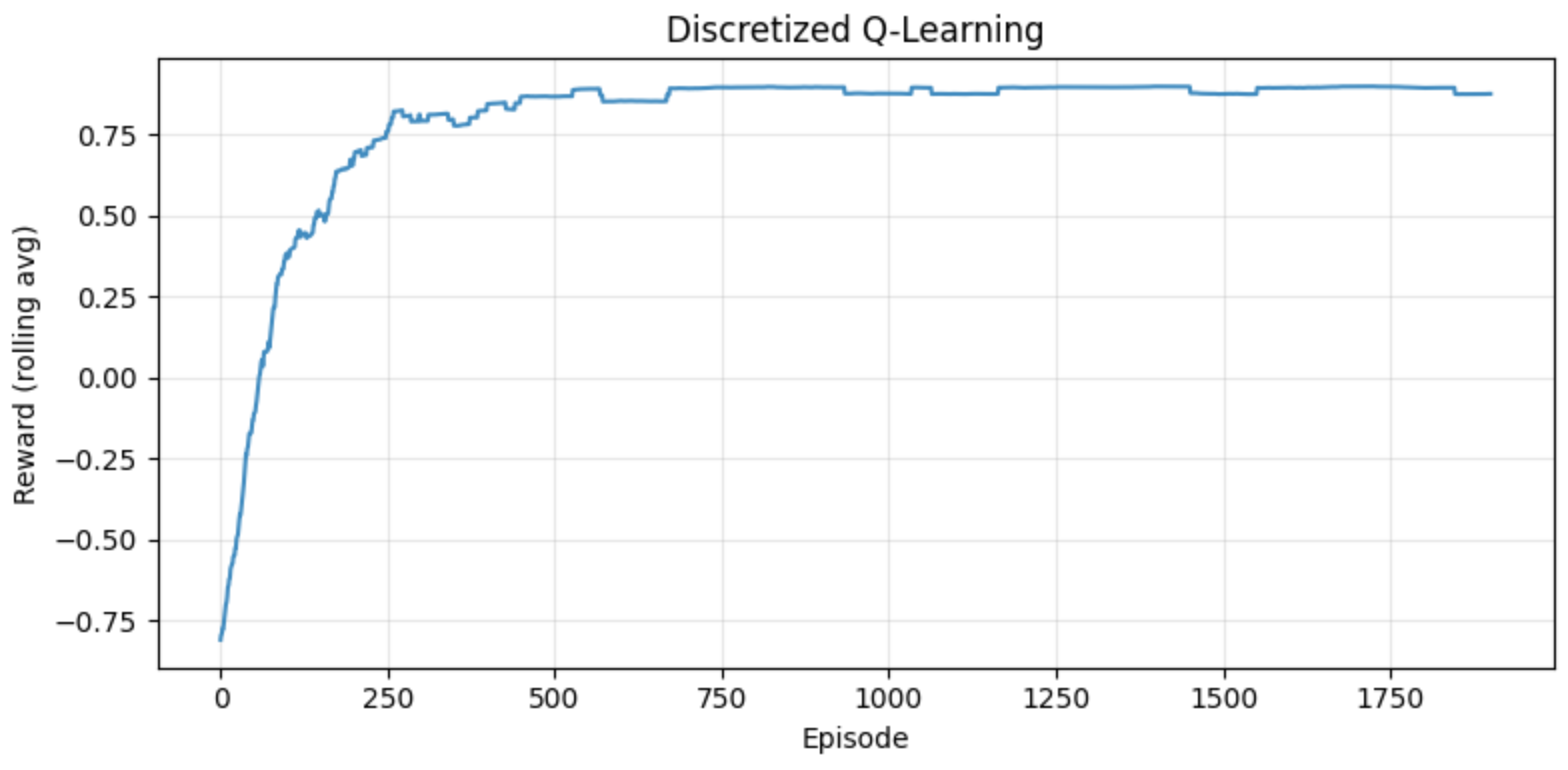
\includegraphics[width=.98\linewidth]{figures/Discretized_Q-learning.png}
\caption{Learning curve for discretized Q-learning in the continuous warehouse environment.}
\label{fig:discretized_q_learning}
\end{figure}

Figure~\ref{fig:discretized_q_learning} summarizes the training behavior of the discretized Q-learning agent.

\begin{itemize}
\item The rolling-average reward trend increases over training, indicating that the discretized Q-learning agent is learning a better policy over time.
\item Early episodes appear noisier (larger return fluctuations), which is consistent with higher exploration at the start of training.
\item As training progresses, the curve becomes smoother and more stable, suggesting convergence toward a consistent behavior.
\item The final part of the curve remains in a high-reward region, implying that a coarse $10 \times 10$ discretization is sufficient to learn effective navigation in this environment.
\item Even with this good final performance, the discretization limits resolution: nearby continuous states share the same bin, which can reduce policy precision near boundaries and hazard-adjacent regions.
\end{itemize}

\subsection{Tile-Coded Linear Q-Learning}

\begin{figure}[htb]
\centering
\includegraphics[width=.98\linewidth]{figures/Tile-Coded_Linear_Q-learning.png}
\caption{Learning curve for tile-coded linear Q-learning in the continuous warehouse environment.}
\label{fig:tile_coded_linear_q_learning}
\end{figure}

Figure~\ref{fig:tile_coded_linear_q_learning} shows the observed training behavior for tile-coded linear Q-learning:

\begin{itemize}
\item The learning curve rises steadily, showing that the tile-coded agent improves policy quality across episodes.
\item Variability is highest early in training, which is expected under high initial exploration and stochastic transitions.
\item The rolling-average trajectory becomes smoother later, indicating more stable value estimates and action selection.
\item Performance plateaus in a high-reward region, suggesting that 8 offset tilings with a $4 \times 4$ base grid are expressive enough for this task.
\item Tile coding achieves useful generalization over nearby continuous states, so it learns faster than purely local lookup behavior.
\item A remaining limitation is feature granularity: states near critical boundaries (especially around the hazard) can still share similar active tiles, which can blur fine control decisions.
\end{itemize}

\subsection{DQN}

\begin{figure}[htb]
\centering
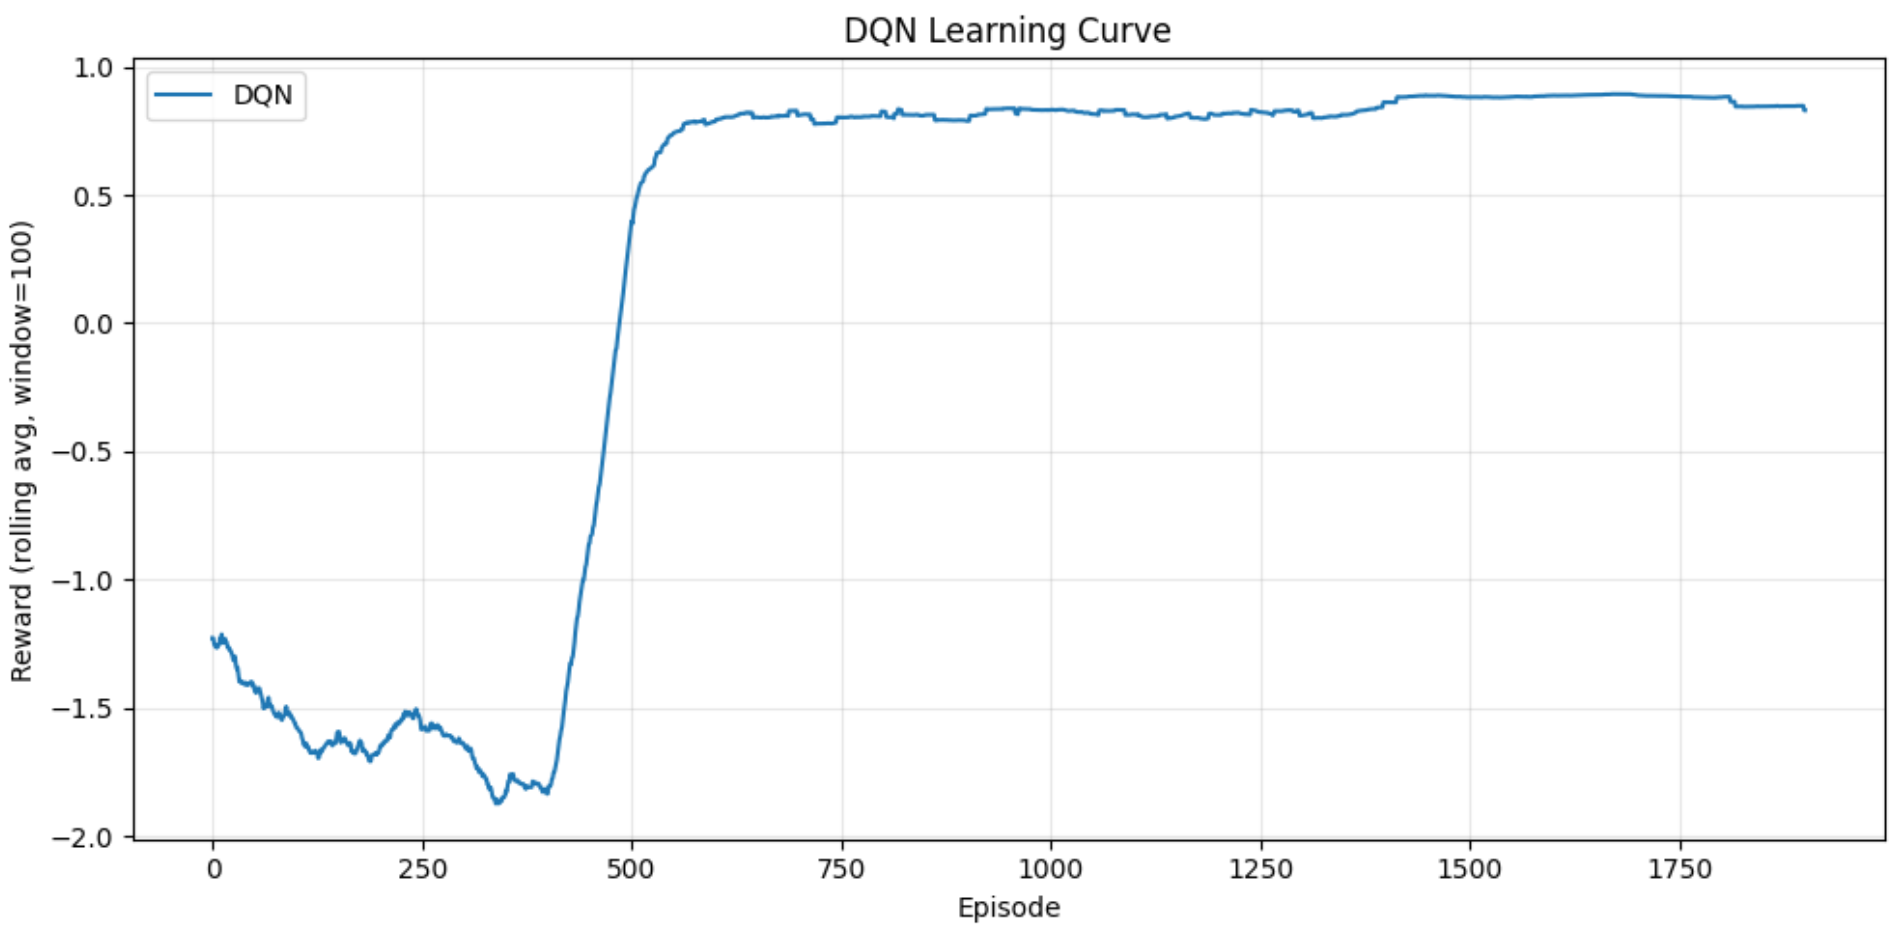
\includegraphics[width=.98\linewidth]{figures/DQN.png}
\caption{Learning curve for DQN in the continuous warehouse environment.}
\label{fig:dqn_learning_curve}
\end{figure}

Figure~\ref{fig:dqn_learning_curve} summarizes the observed DQN learning behavior:

\begin{itemize}
\item The DQN rolling-average reward curve trends upward, indicating that the network is learning increasingly effective action values over training.
\item Early training shows higher variance, which is expected from both stochastic environment transitions and large initial exploration.
\item As episodes progress, the curve becomes smoother and more stable, suggesting that replay-based updates and target-network synchronization improve learning stability.
\item The final part of the trajectory remains in a high-reward region, showing that DQN can learn a strong policy from the full continuous state $(x,y,\theta,v)$.
\item Unlike coarse discretization methods, DQN can represent richer state interactions through learned nonlinear features, which is beneficial in continuous domains.
\item Even so, DQN convergence is sensitive to hyperparameters (learning rate, exploration decay, replay settings, and target update frequency), so stable performance depends on proper tuning.
\end{itemize}

\subsection{Comparisons}

\begin{figure}[htb]
\centering
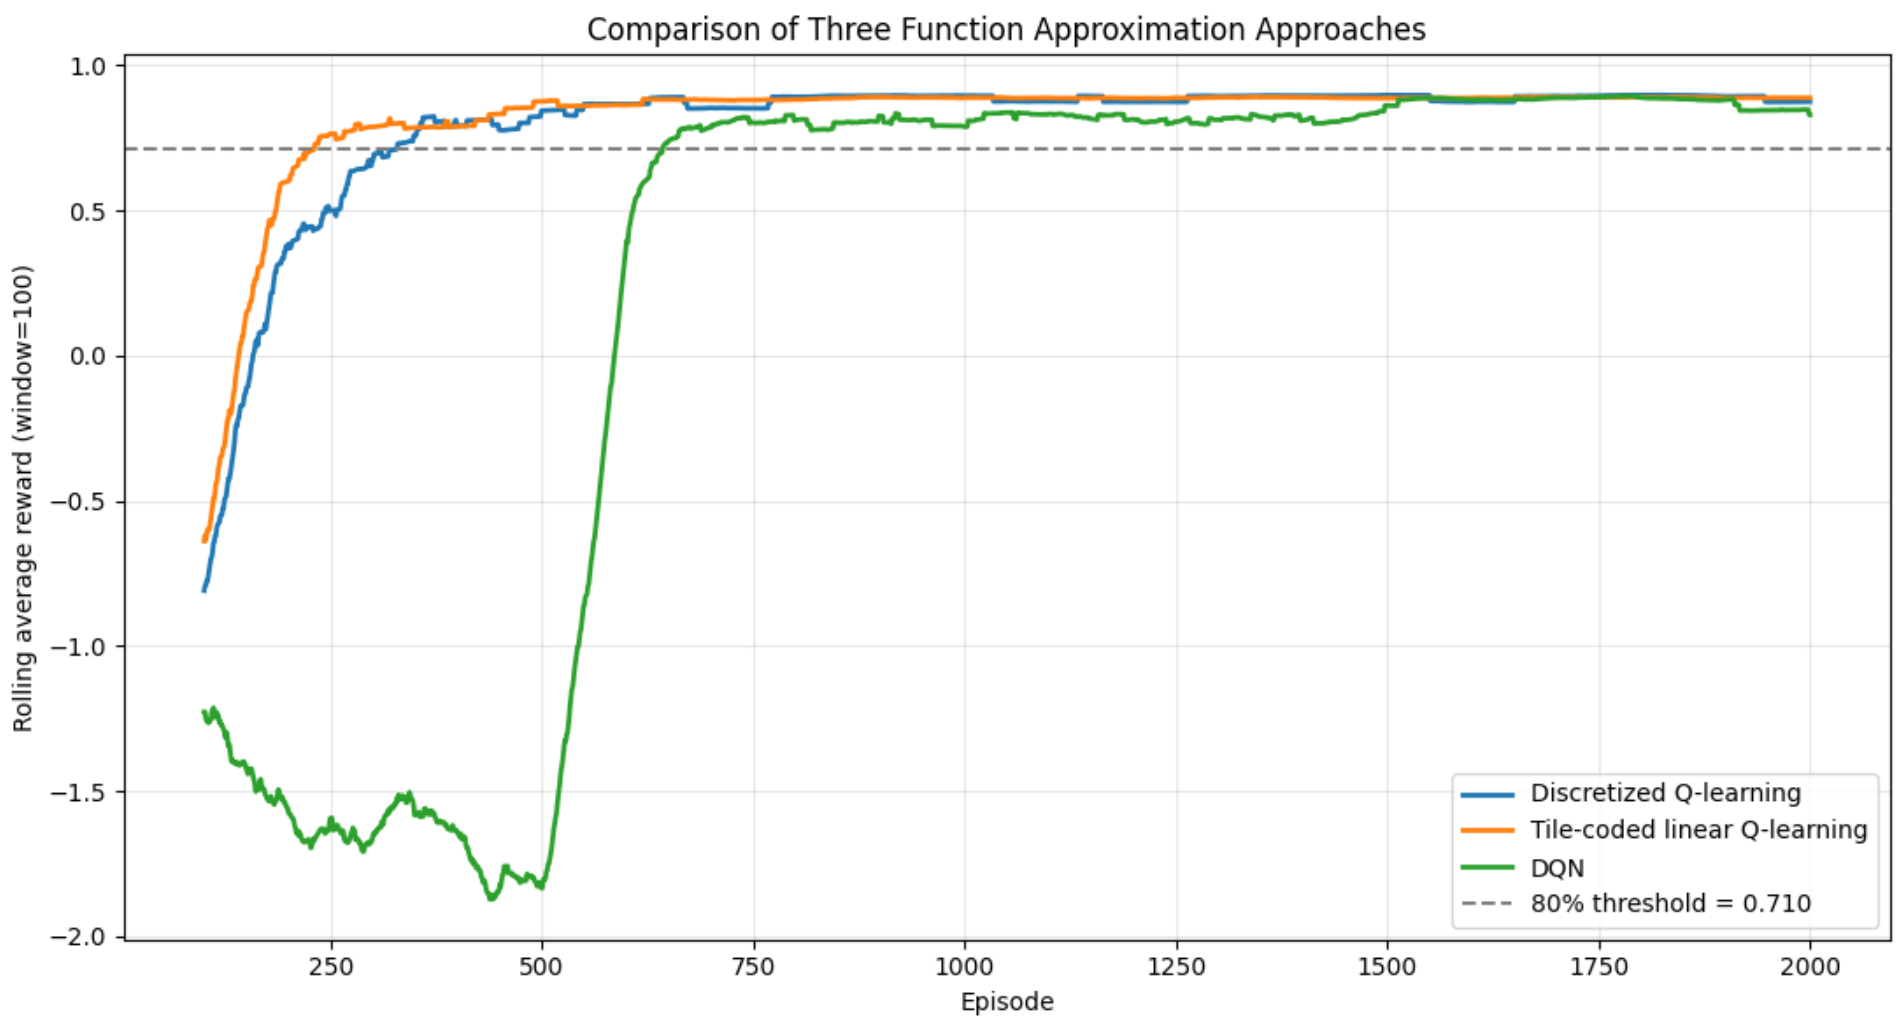
\includegraphics[width=.98\linewidth]{figures/Compare.png}
\caption{Comparison of learning curves and summary performance across discretized Q-learning, tile-coded linear Q-learning, and DQN.}
\label{fig:comparison_all_methods}
\end{figure}

Figure~\ref{fig:comparison_all_methods} summarizes the cross-method comparison using the same rolling-average protocol and performance threshold. Using the reported 80\% optimal-performance threshold of $0.7103$, tile-coded linear Q-learning reached the threshold fastest at 231 episodes, followed by discretized Q-learning at 328 episodes, while DQN required 643 episodes. This indicates that, in this problem setup, the lighter-weight value-function approximators were more sample-efficient early in training than the deeper neural approach.

In terms of asymptotic quality, both tabular-style approximations achieved slightly higher final average reward over the last 200 episodes than DQN: $0.8879$ for tile-coded linear Q-learning and $0.8839$ for discretized Q-learning versus $0.8554$ for DQN. The gap is modest, but it suggests that under the current hyperparameter choices and training budget, DQN did not fully convert its extra representational flexibility into better final return.

Model complexity differed substantially across methods. Discretized Q-learning used 400 parameters, tile-coded linear Q-learning used 800 parameters, and DQN used 4740 parameters. Taken together with the threshold and final-reward metrics, these results show a clear efficiency tradeoff in this experiment: tile-coded linear Q-learning delivered the strongest overall balance of learning speed and final reward with far fewer parameters than DQN, while DQN remained the most expressive option for scaling to richer continuous-state structure beyond this specific task configuration.

\subsection{Ablation study for DQN}

\begin{figure}[htb]
\centering
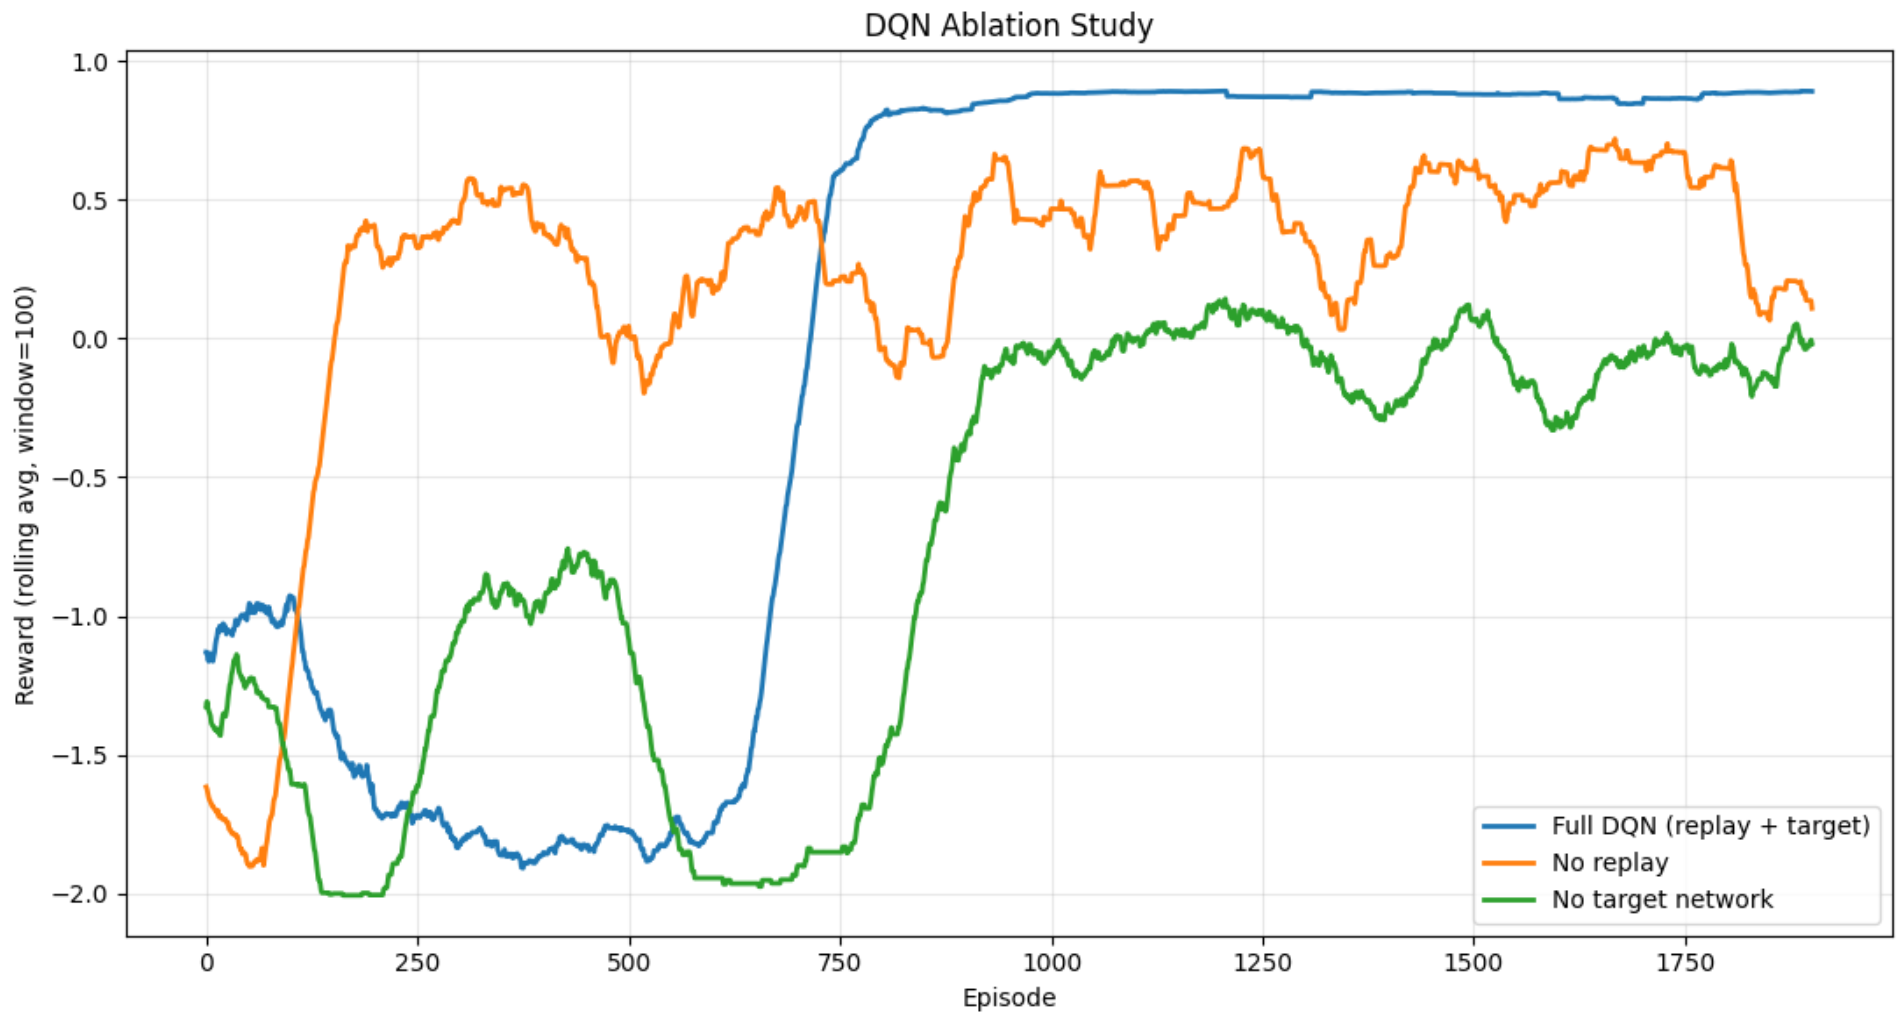
\includegraphics[width=.98\linewidth]{figures/Ablation.png}
\caption{Ablation comparison of full DQN, DQN without replay, and DQN without target network.}
\label{fig:dqn_ablation}
\end{figure}

Figure~\ref{fig:dqn_ablation} evaluates which stabilization components are most important for DQN in this task. The implementation environment was verified before training (Python 3.12.13 with NumPy 2.4.1, Pandas 3.0.1, Matplotlib, scikit-learn 1.8.0, and PyTorch 2.11.0 on CPU), and all runs used the same continuous-warehouse setup to isolate algorithmic differences.

The full DQN variant (experience replay + target network) achieved a final average reward of $0.8862$ over the last 200 episodes, which is consistent with strong and stable convergence. In contrast, removing replay caused a large performance drop to $0.3605$, and removing the target network degraded further to $-0.0594$. These gaps show that both components matter, but the replay buffer has the largest impact on final policy quality under the current training budget.

The stability metric in Figure~\ref{fig:dqn_ablation} supports the same conclusion. Using the standard deviation of tail rolling rewards (lower is better), full DQN achieved $0.0117$, while no-replay and no-target variants rose to $0.1738$ and $0.1028$, respectively. This reproduces the ablation verdict that experience replay contributes more to stability than target-network updates in this experiment, while also confirming that the strongest overall behavior requires both mechanisms together.

These ablation findings align with the broader comparison results: although DQN has higher representational capacity (4740 parameters) than discretized (400) and tile-coded (800) methods, that capacity is only useful when optimization is stabilized. In short, DQN performance here is governed not only by model size but by the effectiveness of replay and target-network design choices.

\section{Conclusion}

Referring to the accompanying Jupyter notebook, we investigated three reinforcement-learning strategies for a \textbf{continuous-state warehouse} task: Discretized Q-learning, Tile-Coded Linear Q-learning, and Deep Q-Networks (DQN).

\subsection*{Key Findings Across Methods}
\begin{itemize}
\item \textbf{All three approaches learned effective policies} and produced upward-trending learning curves, showing that each method can solve the task under a 2000-episode budget.
\item \textbf{Tile-coded linear Q-learning showed the strongest overall balance} of sample efficiency and final return in this experiment.
\item \textbf{DQN did not win by default} despite higher representational power, highlighting that deep methods require careful stabilization and tuning.
\end{itemize}

\subsection*{Quantitative Comparison Summary}
Using the notebook comparison report (80\% threshold = \textbf{0.7103}):

\textbf{Discretized Q-learning}
\begin{itemize}
\item Episodes to 80\%: \textbf{328}
\item Final average reward (last 200): \textbf{0.8839}
\item Parameters: \textbf{400}
\end{itemize}

\textbf{Tile-coded linear Q-learning}
\begin{itemize}
\item Episodes to 80\%: \textbf{231} (fastest)
\item Final average reward (last 200): \textbf{0.8879} (best)
\item Parameters: \textbf{800}
\end{itemize}

\textbf{DQN}
\begin{itemize}
\item Episodes to 80\%: \textbf{643} (slowest)
\item Final average reward (last 200): \textbf{0.8554}
\item Parameters: \textbf{4740}
\end{itemize}

These numbers show a clear tradeoff: for this specific environment and training horizon, the simpler structured approximators (especially tile coding) were more data-efficient and slightly stronger in final return than the deeper model.

\subsection*{Interpretation of Representation Choices}
\begin{itemize}
\item \textbf{Discretized Q-learning} works well as a strong baseline, but coarse binning can merge distinct nearby states and reduce control precision near critical regions (for example, around hazards and boundaries).
\item \textbf{Tile coding} improves on this by introducing overlapping local generalization while keeping updates linear and stable; this likely explains its faster convergence and top final performance here.
\item \textbf{DQN} can represent richer nonlinear interactions over the full state, which is a major long-term advantage for higher-dimensional or more complex continuous tasks, but the current results show that this flexibility only helps when optimization is well stabilized.
\end{itemize}

\subsection*{DQN Ablation Conclusions}
The ablation study directly tested DQN stability components:
\begin{itemize}
\item Full DQN (replay + target): final-200 reward \textbf{0.8862}, tail-std \textbf{0.0117}
\item No replay: final-200 reward \textbf{0.3605}, tail-std \textbf{0.1738}
\item No target network: final-200 reward \textbf{-0.0594}, tail-std \textbf{0.1028}
\end{itemize}

The verdict from both performance and stability metrics is that \textbf{experience replay contributed more to stability} than the target network in this setup, though both were important for reliable learning.

\subsection*{Overall Takeaway}
For this continuous warehouse task, \textbf{tile-coded linear Q-learning provided the best practical balance} of speed, stability, and return with modest parameter count. \textbf{DQN remained the most expressive method}, but its advantage did not fully materialize under the current hyperparameters and budget without strong stabilization. The broader lesson is that in continuous RL, model capacity alone is not enough: \textbf{representation, optimization stability, and hyperparameter design jointly determine performance}.

%%% References -------------------------

\nocite{*}
\bibliographystyle{plainnat}
\bibliography{report}


%%% Appendices -------------------------

\end{document}  